\documentclass[11pt, a4paper]{article}

\usepackage[utf8]{inputenc}
\usepackage{geometry}
\geometry{top=1in, bottom=1in, left=1in, right=1in}
\usepackage{amsmath}
\usepackage{amssymb}
\usepackage{verbatim}
\usepackage{xcolor}
\usepackage{graphicx}

% R code styling
\usepackage{listings}
\lstset{
    basicstyle=\ttfamily\small,
    breaklines=true,
    backgroundcolor=\color{gray!10},
    frame=single,
    numbers=none,
    keepspaces=true
}

\title{\textbf{SM\&I - Test 1}}
\author{Yuchen Sun / 24220003069}
\date{\today}

\begin{document}

\maketitle

% ---------------------------------------------------------
% QUESTION 1
% ---------------------------------------------------------
\section*{Question 1}

\subsection*{R Script and Output}
\begin{lstlisting}
# Question 1: Two-sample inference for porosity means

n1 <- 40; ybar1 <- 0.22; s1_sq <- 0.0010
n2 <- 35; ybar2 <- 0.17; s2_sq <- 0.0020

diff <- ybar1 - ybar2
SE <- sqrt(s1_sq/n1 + s2_sq/n2)

# Welch-Satterthwaite degrees of freedom
df_num <- (s1_sq/n1 + s2_sq/n2)^2
df_den <- (s1_sq/n1)^2/(n1-1) + (s2_sq/n2)^2/(n2-1)
df <- df_num / df_den

# 95% CI
t_crit <- qt(0.975, df)
CI_lower <- diff - t_crit * SE
CI_upper <- diff + t_crit * SE

# One-sided test H0: mu1-mu2 <= 0.02 vs H1: > 0.02
delta0 <- 0.02
t_stat <- (diff - delta0) / SE
p_value <- 1 - pt(t_stat, df)

cat("Point estimate =", diff, "\n")
cat("SE =", SE, "\n")
cat("df =", df, "\n")
cat("95% CI: (", CI_lower, ",", CI_upper, ")\n")
cat("t-statistic =", t_stat, "\n")
cat("One-tailed p-value =", p_value, "\n")
if (p_value < 0.05) cat("Reject H0: mu1 - mu2 > 0.02\n")
\end{lstlisting}

\textbf{Console Output:}
\begin{lstlisting}
Point estimate = 0.05 
SE = 0.00906327
df = 60.21064 
95% CI: ( 0.03187207 , 0.06812793 )
t-statistic = 3.310064 
One-tailed p-value = 0.0007894957 
Reject H0: mu1 - mu2 > 0.02
\end{lstlisting}

\subsection*{Answers and Interpretation}

\textbf{(a) 95\% Confidence Interval for $\mu_1 - \mu_2$}\\
Using the Welch two-sample t-interval (unequal variances), the estimated difference is $\hat{\mu}_1-\hat{\mu}_2 = 0.05$ with standard error $0.00906$ and $60.2$ degrees of freedom. The 95\% confidence interval is 
\[
(0.0319,\; 0.0681).
\]
We are 95\% confident that the true difference in mean porosity (lab 1 – lab 2) lies between $0.0319$ and $0.0681$.

\textbf{(b) Hypothesis Test}\\
We test 
\[
H_0: \mu_1-\mu_2 \le 0.02 \quad \text{vs.} \quad H_1: \mu_1-\mu_2 > 0.02
\]
at the 5\% significance level. The test statistic is $t = 3.310$ with $60.2$ df, giving a one-tailed p-value of $0.0008$. Since $p < 0.05$, we reject $H_0$. There is sufficient evidence to conclude that the difference between the population means is greater than $0.02$.

\textbf{(c) Interpretation}\\
The 95\% confidence interval lies entirely above $0.02$ (lower bound $0.0319 > 0.02$), which aligns with the rejection of $H_0$ in part (b). Thus, laboratory 1 produces solid copper with a statistically significantly higher mean porosity than laboratory 2, and the difference exceeds $0.02$ at the 5\% significance level.

% ---------------------------------------------------------
% QUESTION 2
% ---------------------------------------------------------
\section*{Question 2}

\subsection*{R Script and Output}
\begin{lstlisting}
# Question 2: Linear regression of Horsepower on Cylinder Volume

cyl_vol <- c(1.8, 1.5, 2.0, 2.5, 1.8, 2.5, 1.6, 1.5)
horsepower <- c(51, 51, 115, 150, 126, 150, 118, 106)

model <- lm(horsepower ~ cyl_vol)
summary(model)

# Scatter plot with regression line
plot(cyl_vol, horsepower, 
     xlab = "Cylinder Volume (L)", 
     ylab = "Horsepower",
     main = "Horsepower vs. Engine Size")
abline(model, col = "red", lwd = 2)

# Estimate mean horsepower for 1.9 L
new_data <- data.frame(cyl_vol = 1.9)
predict(model, new_data, interval = "confidence", level = 0.95)
\end{lstlisting}

\textbf{Console Output:}
\begin{lstlisting}
Call:
lm(formula = horsepower ~ cyl_vol)

Residuals:
    Min      1Q  Median      3Q     Max 
-50.858  -7.746   2.522  23.806  29.177 

Coefficients:
            Estimate Std. Error t value Pr(>|t|)  
(Intercept)   -15.45      54.84  -0.282   0.7876  
cyl_vol        65.17      28.30   2.303   0.0609 .
---
Signif. codes:  0 ‘***’ 0.001 ‘**’ 0.01 ‘*’ 0.05 ‘.’ 0.1 ‘ ’ 1

Residual standard error: 30.48 on 6 degrees of freedom
Multiple R-squared:  0.4692,	Adjusted R-squared:  0.3807 
F-statistic: 5.303 on 1 and 6 DF,  p-value: 0.06087

      fit      lwr      upr
1 108.375 82.00477 134.7452
\end{lstlisting}

\begin{figure}[htbp]
\centering
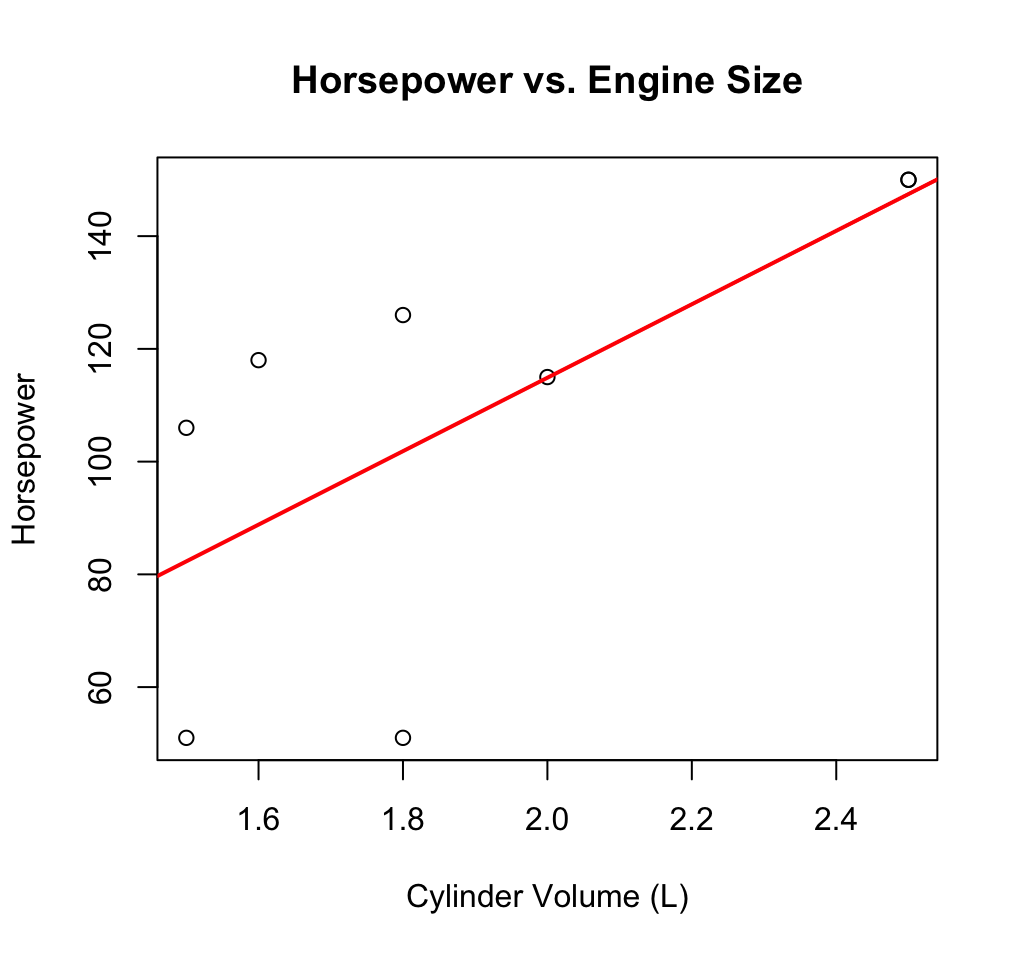
\includegraphics[width=0.7\textwidth]{1.png}
\caption{Scatter plot of Horsepower vs. Cylinder Volume with the least‑squares line.}
\label{fig:q2plot}
\end{figure}

\subsection*{Answers}

\textbf{(a) Least‑squares line}\\
Based on the R output, the estimated intercept $b_0 = -15.45$ and slope $b_1 = 65.17$. The regression equation is
\[
\widehat{\text{Horsepower}} = -15.45 + 65.17 \times \text{Cylinder Volume (L)}.
\]

\textbf{(b) Graph}\\
The scatter plot (Figure 1) shows a moderate positive linear relationship. The least‑squares line (red) captures the general upward trend, but the fit is not very strong: the residual standard error is $30.48$, and $R^2 = 0.4692$ indicates that only about $46.9\%$ of the variability in horsepower is explained by cylinder volume. The p‑value for the slope is $0.0609$, which is marginally above $0.05$, suggesting that the relationship is not statistically significant at the conventional 5\% level.

\textbf{(c) Estimated mean horsepower for 1.9 L}\\
For a cylinder volume of $1.9$ L, the predicted mean horsepower is $108.38$. The 95\% confidence interval for the true mean horsepower of all such automobiles is $(82.00,\; 134.75)$.

\end{document}